\section{Introduction}

This document is a proposal for the research project I will conduct for my Master's thesis during the spring of 2016. It begins by listing core aims and objectives for the project in terms of what I seek to deliver. It then suggests a research approach to achieve this goal, and finally presents a brief project plan.

My \textbf{overarching research question} is how we can best compare several strategies for automating deployment in an environment with many teams and services, and pick or compose a strategy that suits the context.

My motivation for this project comes from the action design research-like work I completed in the Master programme's practise period module. During this project, I identified automated deployment of microservices as a time-consuming and error-prone task that is often repeated for each new service.

A brief literature search will show that much work has already been done on both automated deployment and microservices individually, such as \autocite{virmani:2015}, \autocite{stolberg}, \autocite{savchenko:2015}, and \autocite{le:2015}. However, it appears from the literature review I conducted then that little work is completed on automated deployment in a microservice context. This must be shown explicitly in my thesis.

\section{Aim and objectives}

As mentioned in the previous section, deployment in a microservice context is a task that is both difficult and time-consuming. My \textbf{overall aim} for the research is to help simplify this process through three \textbf{key goals}:

\begin{enumerate}
  \item Providing further insight into how implementation of automated microservice deployment;
  \item Creating a framework for analysing different strategies for automated deployment in the future; and
  \item Conducting an analysis of a few popular strategies for automated deployment.
\end{enumerate}

In order to reach these goals, my \textbf{specific objectives} are:

\begin{enumerate}
  \item Reviewing the existing literature on deployment automation (in this context commonly referred to as continuous integration or continuous delivery), the microservice architectural style in general, how they can be tied together;
  \item Establishing relevance by learning which factors are important to the industry;
  \item Developing an initial framework for analysing strategies based on the findings from the literature review (1) and the case study (2);
  \item Testing, analysing, and comparing some popular deployment automation strategies using the framework from (3) to simplify picking or composing a strategy and validate and mature the framework.
\end{enumerate}

\section{Research approach}

I suggest triangulating two research strategies:

\begin{enumerate}
  \item A case study to establish which factors are important to the industry to supplement the literature review; and
  \item A design science research \autocite{vaishnavi:2015} (specifically, design \& creation \autocite{oates:2006}) project to test various deployment strategies.
\end{enumerate}

\subsection{Case study: What is important to FINN.no?}

Together with data from a literature review, I will build a first version of a framework for analysing the pros and cons of various strategies. This framework will be the key artefact of this thesis. In order to find which factors are important to the industry, I will conduct a case study at FINN.no. Using interviews and a document analysis for data generation, I will gather data on the company's own analysis of various strategies and how they plan to implement their own. I will interview (at least):

\begin{enumerate}
  \item Key members of the cloud migration team responsible for implementing containers to understand which efforts are being made;
  \item The team lead for one of FINN's teams that has completely deviated from the company's standard way to do deployment;
  \item The person(s) responsible for the containerisation in order to uncover why the effort is made and which factors determine which strategy is selected; and
  \item A key member of the cloud migration team to polish and verify my findings.
\end{enumerate}

These interviews will provide insight into which strategies are actually being used for automated deployment, and how they are composed. This initial version of the framework then be used to analyse some implementations based on the next step.

All the listed interviews are already agreed upon by FINN.no, so the risk of not being able to gather data is relatively small. Additionally, if it proves unfeasible to gather data required to build a framework, I will simply need to lean more heavily toward my findings during the literature review. Thus, even if this phase should yield few results, the project can continue. The obvious downside of this outcome is that the industry is not necessarily represented strongly in building the framework, which makes it harder to establish a strong relevance.

\subsection{Implementation through design science research}

In this final phase of the project, I will iteratively improve the analysis framework for analysing deployment automation strategies derived from the literature review and case study.

In order to test strategies, I will need to build some relatively simple microservices that can be used for deployment. I will write these services in a few popular programming languages using frameworks commonly used by the industry to improve the study's generalisability. I expect to use an Infrastructure as a Service\footnote{A service where the hardware and network are abstracted away, but one receives access directly to the operating system(s).} such as Amazon Web Services (AWS)\footnote{\url{https://aws.amazon.com/}} to set up a test environment.

The first major revision of the framework will come from implementing and testing a strategy close to the one FINN is committed to. This test will likely raise several new concerns to include in the framework, as the issues must be explicitly addressed. The implementation of a few other strategies will both help improve the analysis framework and provide data that can help practitioners select a strategy that suits them. Practitioners can even compose their own strategies and compare them using the framework.

I will iteratively add to the total number of strategies I test; if I am able to implement and test a first strategy, this phase will already have yielded useful results. Given the time schedule presented in the next section, this should not be a high risk. However, the study's validity and generalisability are highly dependent on more than one implemented and evaluated strategy, as the key artefact from this phase is a comparison of various strategies.

\section{Project plan}

Figure \ref{fig:plan-with-dates} presents a Gantt diagram-like overview of the project's key milestones and my other activities for the semester with rough dates.

\begin{figure}[H]
    \label{fig:plan-with-dates}
\centerline{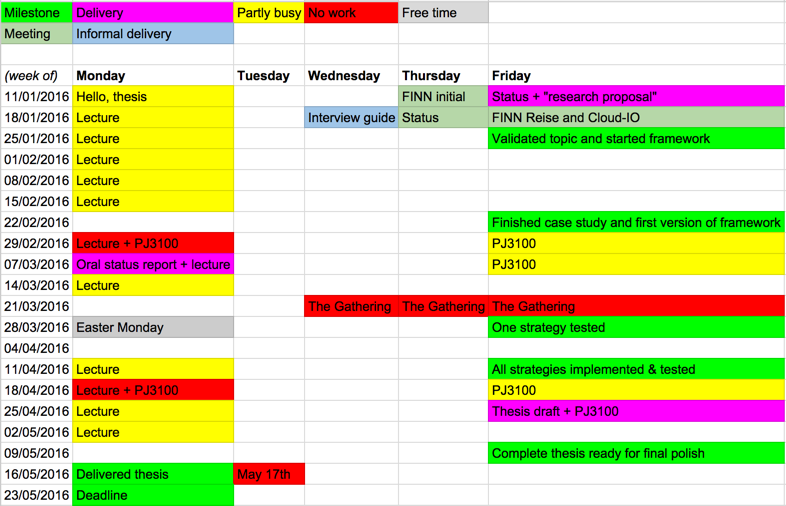
\includegraphics[scale=0.6]{plan-with-dates}}
    \caption{Plan with dates}
\end{figure}

The key points are as follows:

\begin{enumerate}
  \item The preliminary case study and the initial version of the analysis framework derived from a literature review and the case study should be completed by the end of February.
  \item The test infrastructure and services, as well as the first deployment automation strategy should be implemented and tested by the end of March.
  \item All 3--4 strategies should be implemented, tested, and compared mid-April.
  \item The first complete draft of the thesis should be ready by the end of April.
  \item The thesis should be polished and almost ready for delivery mid-May.
\end{enumerate}

The plan is intentionally very rough, and is only meant to be a brief overview. The document is live, and will be altered and updated as milestones are met earlier or later than expected. As touched upon in section 3.2, my plan for implementation work and comparison takes into account the possibility of only being able to test one or two strategies by working iteratively.

\subsection{Risk analysis}

Figure \ref{fig:risk-analysis} presents an initial risk analysis for the project. Risks are ordered by risk points determined by probability (0-1) * consequence (0-10). Each risk has associated proactive and reactive steps.

\begin{figure}[H]
    \label{fig:risk-analysis}
\centerline{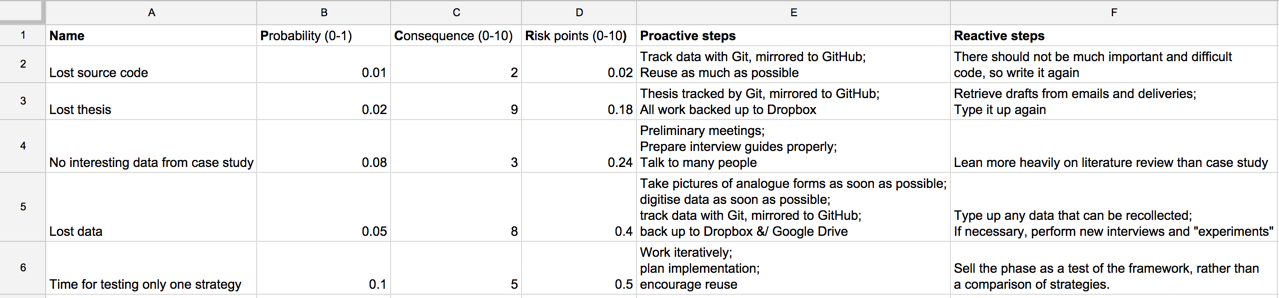
\includegraphics[scale=0.45]{risk-analysis}}
    \caption{Risk analysis by risk points (R = P * C)}
\end{figure}

I have tried to keep the plan as practical as possible. As new risks are discovered, the document\footnote{Live version available at \url{https://docs.google.com/spreadsheets/d/1ugcNV14-5exXiV5IFfFDR11uEIXZbvikrce4JsCb71U/edit?usp=sharing}} will be updated.

\section{Potential titles}

So far, I only have one potential title. Suggestions will be kept in and added to a live document during the writing process.

\begin{itemize}
  \item A comparison of automated deployment strategies
\end{itemize}
